\label{par:analyser_operateurs_nagumo}
L'équation de Nagumo (ou FitzHugh-Nagumo) est issue de modèles de transmission de l'information nerveuse \cite{FITZHUGH1961445}.
L'étude travaille sur la forme spatiale de l'équation \cite{keener1998mathematical} avec un terme de réaction cubique introduisant de la non-linéarité:
\begin{align}
    \dt{u} = \underbrace{D \dxx{u}}_{\text{diffusion}}
            - \underbrace{ku(1-u^2)}_{\text{réaction}}.
\end{align}
\subsubsection{Solutions Analytiques}
L'équation admet des solutions propagatives sous la forme\footnote{C'est une sigmoïde, qui se propage à vitesse $\sqrt{\frac{kD}{2}}$ \cite{duart2011}.}:
\begin{align}
    \label{eq:sol_nagumo}
    u(x-ct) = \frac{e^{
        \sqrt{\frac{k}{2D}} \bigl((x-x_0) - ct \bigr)}
    }
    {1 + e^{
        -\sqrt{\frac{k}{2D}} \bigl((x-x_0) - ct \bigr)}
    }
\end{align}
Avec : $c = \sqrt{\frac{kD}{2}}$ et $x_0$ le point de départ de l'onde.\\
Ainsi, le produit $kD$ fixe la vitesse et le ratio $\frac{k}{D}$ la magnitude du gradient d'espace.

\begin{figure}[htbp]
    \centering
    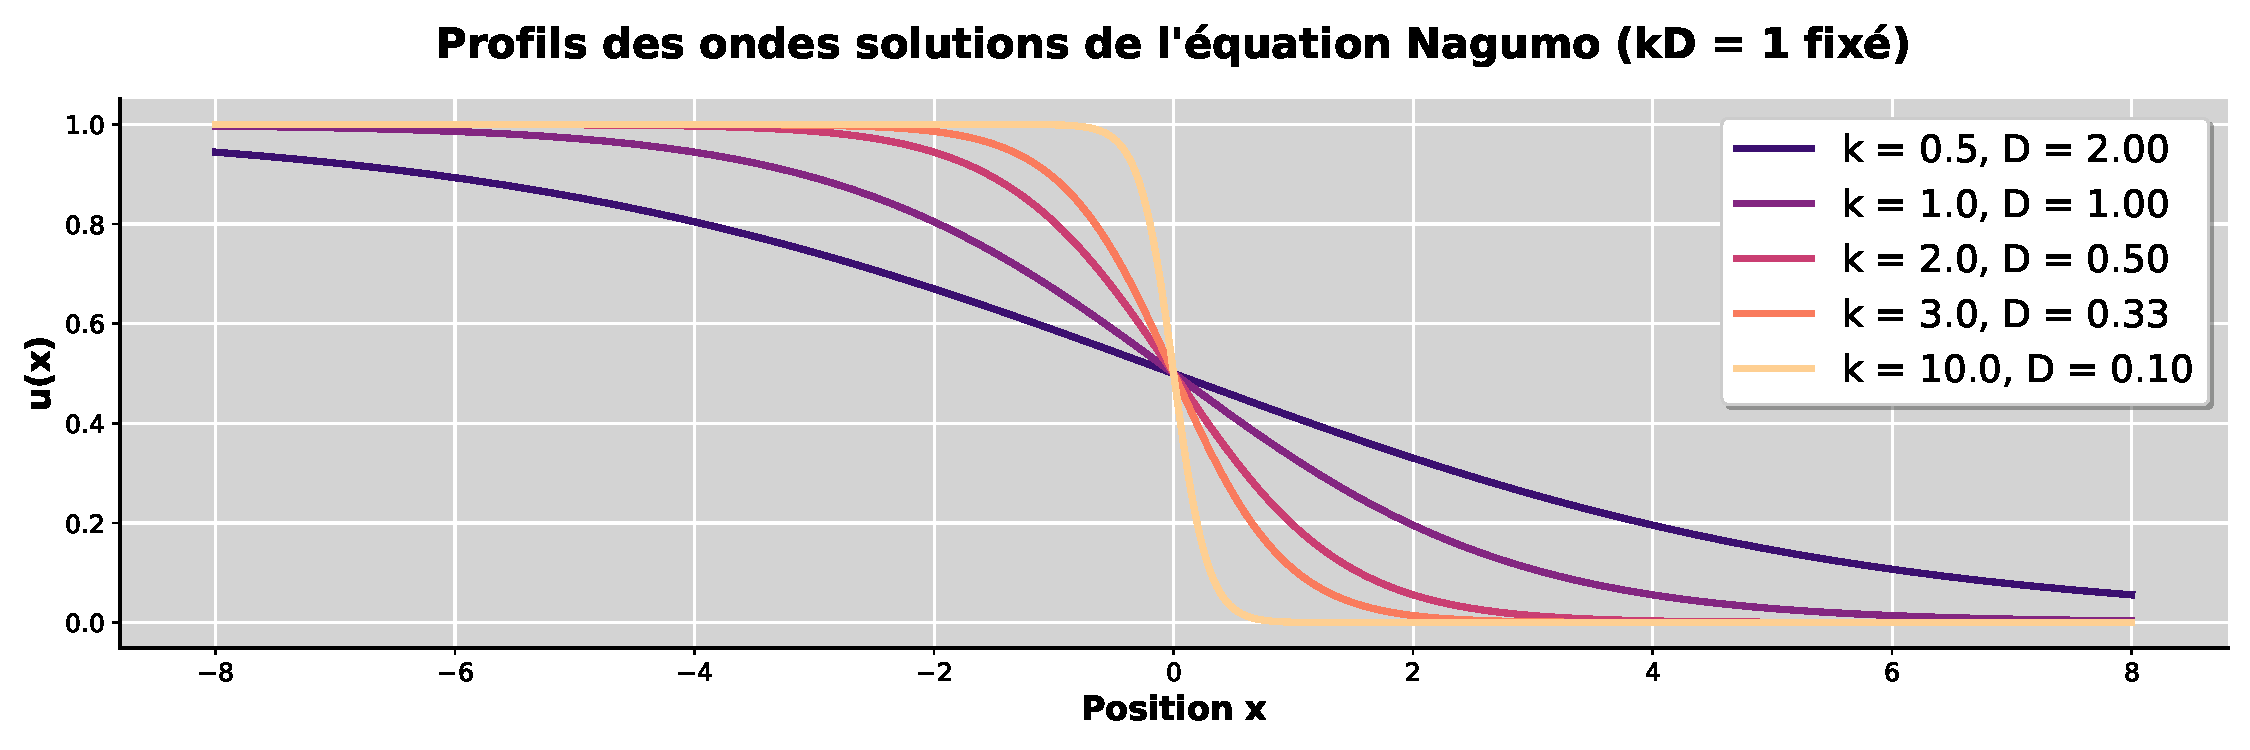
\includegraphics[width=\textwidth]{media/4_travail/2_nagumo/profils_nagumo.pdf}
    \caption{Profils des ondes solutions de l'équation de Nagumo pour différents ratios $k/D$ avec le produit $kD = 1$ fixé (c'est à dire à vitesse fixée). L'augmentation du ratio k/D accentue le gradient spatial.}
    \label{fig:profils_nagumo}
\end{figure}

\subsubsection{Analyse des opérateurs}
Un analyse des deux opérateurs de l'EDP est nécessaire pur en saisir les enjeux.
\textit{L'opérateur de diffusion} est non-local et, discrétisé à l'ordre deux par $n$ points et un pas $\Delta x$, les valeurs propres associées sont 
$\left\{ \frac{2D}{\Delta x^2} \left(\cos \frac{p\pi}{n+1} - 1\right) \mid p \in \{1,\dots,n\} \right\}$ \cite{bouchet2020laplacien}, 
ainsi la raideur du terme de diffusion croit linéairement avec le coefficient de diffusion $D$ et de manière quadratique avec la finesse du maillage $1/\Delta x$.
En effet les valeurs propres sont négatives et:
\begin{align}
    \max_p \vert\cos \frac{p\pi}{n+1} - 1 \vert &\sim 2,\\
    \min_p \vert \cos \frac{p\pi}{n+1} - 1 \vert &\sim \frac{1}{2}\Bigl( \frac{\pi}{n+1} \Bigr)^2.
\end{align}
Et donc:
\begin{align}
    \frac{\max_p \vert 1 - \cos \frac{p\pi}{n+1} \vert}{\min_p \vert 1 - \cos \frac{p\pi}{n+1} \vert} \approx n^2\propto \left(\frac{1}{\Delta x}\right)^2.
\end{align}
Concernant \textit{le terme de réaction}, en choisissant un état initial correspondant à \ref{eq:sol_nagumo},
la solution reste entre 0 et 1. Ainsi le terme de réaction est local en espace, et ses valeurs propres sont comprises entre $-k$ et $2k$.
En fonction de la valeur de $u$, la réaction se comporte localement (dans le temps et l'espace) comme une relaxation de temps caractéristique $\tau \sim \frac{1}{k}$ ou comme une explosion de temps 
caractéristique $\tau \sim \frac{1}{2k}$, en effet: 
\begin{align}
    \text{Terme de réaction: }&R(u) = ku(1-u^2),\\
    \text{Valeurs propres de la réaction: }&R'(u) = k (1 - 3u^2).
\end{align}
Pour les valeurs étudiés, $k \leq 20$, la réaction reste ainsi peu raide par rapport au "vraies" réactions chimiques (il faut avoir conscience de cette 
différence pour considérer ce cas test de la bonne manière, ici la réaction est le terme le moins raide alors que sur des "vrais" applications, ce n'est pas le cas).
\begin{figure}[htbp]
    \centering
    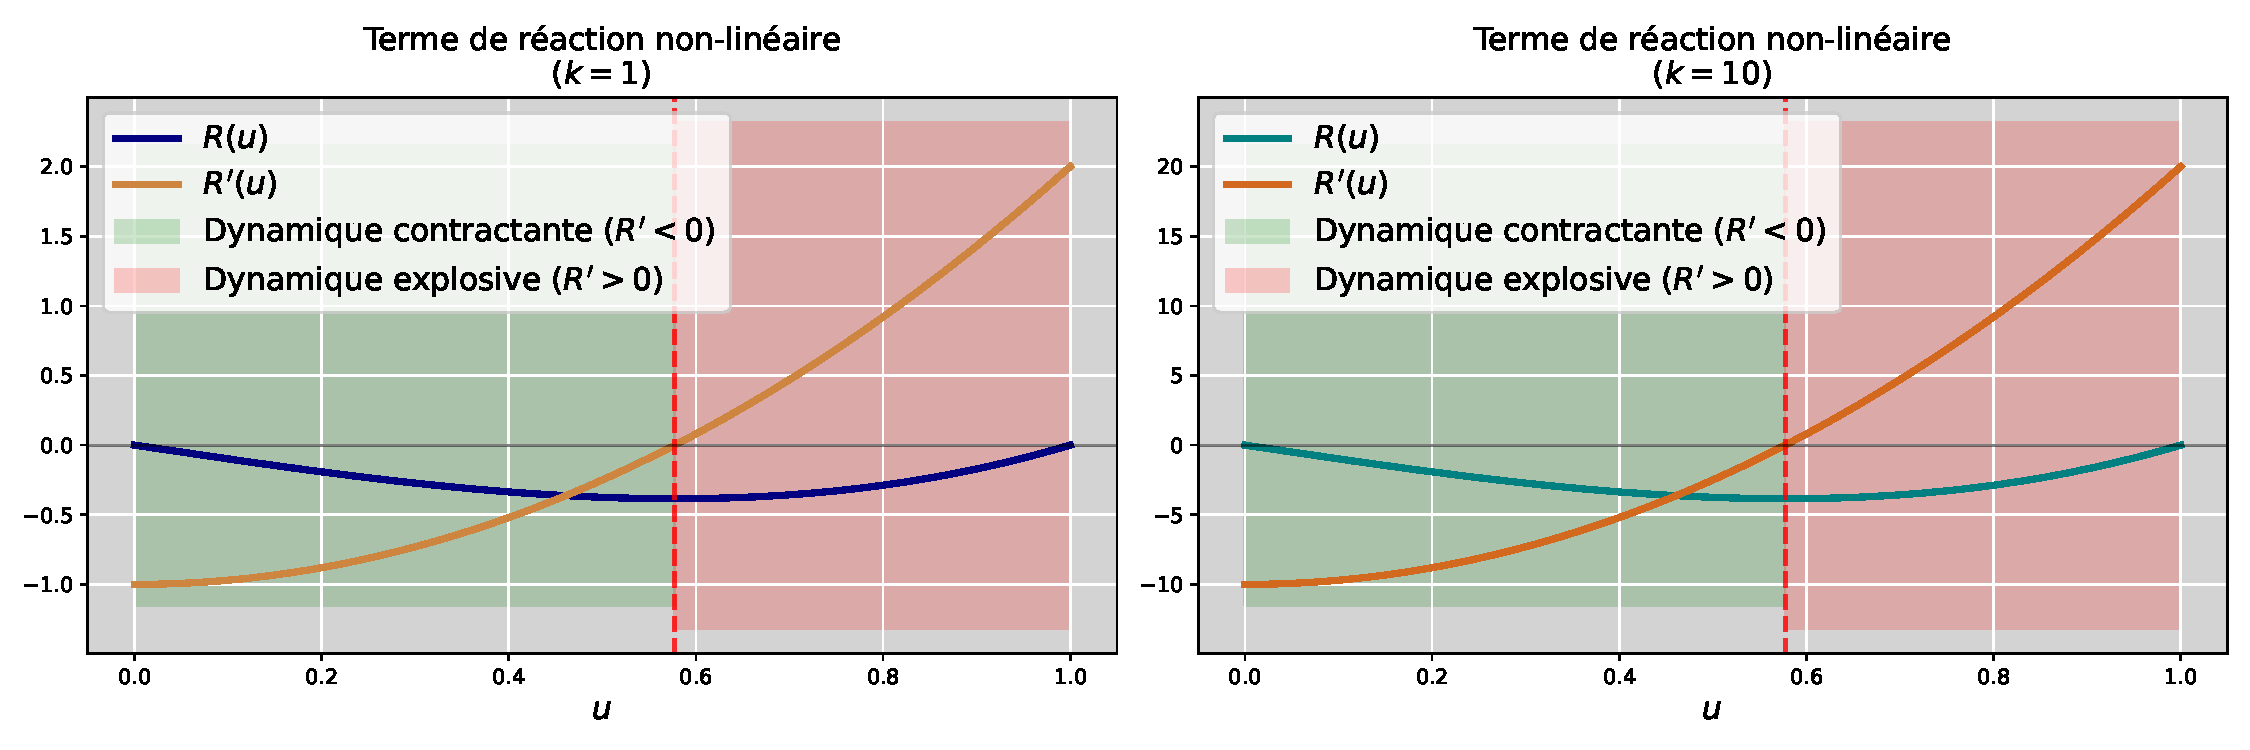
\includegraphics[width=\textwidth]{media/4_travail/2_nagumo/raideur_reaction_nagumo.pdf}
    \caption{Plage de valeurs du terme de réaction non-linéaire et de sa différentielle pour deux coefficients de réactions: $k=1$ et $k=10$.}
    \label{fig:raideur_reaction_nagumo}
\end{figure}

\subsubsection{Conclusion sur l'équation de Nagumo}
Ainsi l'équation de Nagumo, présente un terme de réaction\footnote{à noter qu'il n'est pas raide, comparé aux termes de réaction rencontrés en combustion.},
et un terme de diffusion. Cette équation fait émerger un front d'onde\footnote{Cela permet de tester le comportement de la multi-résolution adaptative.} et dispose de deux paramètre $k$ et $D$ pour piloter aisément les propriétés des solutions.
Cela en fait donc une équation-test de choix pour étudier le comportement de diverses méthodes dédiées aux équations d'advections-réaction-diffusion. 